%=============================================================================%
% Preamble
%=============================================================================%
% Libraries

\documentclass[xcolor=table]{beamer}
%\usepackage{beamerthemeshadow}
\usepackage{helvet}
\usepackage[]{graphicx}
\usepackage{array}
\usepackage{color}
\definecolor{dkgreen}{rgb}{0,0.6,0}
\definecolor{gray}{rgb}{0.5,0.5,0.5}
\definecolor{mauve}{rgb}{0.58,0,0.82}
\definecolor{deepblue}{rgb}{0,0,0.5}
\definecolor{deepred}{rgb}{0.6,0,0}
\definecolor{deepgreen}{rgb}{0,0.5,0}
\definecolor{lightgray}{rgb}{0.92,0.92,0.92}
\usepackage{listings} % to insert code
\usepackage{textpos} % textblock
\usepackage{hyperref}
\hypersetup{colorlinks=true, urlcolor=blue, linkcolor=black} 
% Listing set up
% bash
\lstdefinestyle{bash}{
language=bash,                     % the language of the code
basicstyle=\scriptsize\ttfamily,       % the size of the fonts that are used for the code
numbers=none,%left,                   % where to put the line-numbers
numberstyle=\tiny\color{gray},  % the style that is used for the line-numbers
stepnumber=1,                   % the step between two line-numbers. If it's 1, each line
                          % will be numbered
numbersep=5pt,                  % how far the line-numbers are from the code
backgroundcolor=\color{lightgray},  % choose the background color. You must add \usepackage{color}
showspaces=false,               % show spaces adding particular underscores
showstringspaces=false,         % underline spaces within strings
showtabs=false,                 % show tabs within strings adding particular underscores
frame=lines,%single,                   % adds a frame around the code
rulecolor=\color{black},        % if not set, the frame-color may be changed on line-breaks within not-black text (e.g. commens (green here))
tabsize=2,                      % sets default tabsize to 2 spaces
captionpos=b,                   % sets the caption-position to bottom
breaklines=true,                % sets automatic line breaking
breakatwhitespace=false,        % sets if automatic breaks should only happen at whitespace
title=\lstname,                 % show the filename of files included with \lstinputlisting;
                          % also try caption instead of title
keywordstyle=\color{blue},      % keyword style
commentstyle=\color{dkgreen},   % comment style
stringstyle=\color{mauve},      % string literal style
escapeinside={\%*}{*)},         % if you want to add a comment within your code
morekeywords={}            % if you want to add more keywords to the set
}

\lstdefinestyle{python}{
language=python,
formfeed=\newpage,
basicstyle=\scriptsize\ttfamily,
commentstyle=\color{deepgreen},%\color{gray},
numbers=left,
numberstyle=\tiny\color{gray},
stepnumber=1,
numbersep=5pt,
backgroundcolor=\color{lightgray},%\color{white},
showspaces=false,
showstringspaces=false,
showtabs=false,
frame=lines,
tabsize=4,
captionpos=b,
breaklines=true,
breakatwhitespace=false,
title=\lstname,
escapeinside={},
keywordstyle=\color{deepblue},
emphstyle=\color{deepred},
stringstyle=\color{deepgreen}
%morekeywords={models, lambda, forms}
}

\graphicspath{ {../img/} }

\begin{document}
\title{Python for Scientific Research}   
\author{Bram Kuijper}
\institute[]{University of Exeter, Penryn Campus, UK}
\titlegraphic{
\hfill

\includegraphics[width=\textwidth, keepaspectratio]{logo.jpg}}

\frame{\titlepage} 
\begin{frame}{Acknowledgements}
\begin{itemize}\addtolength{\itemsep}{\baselineskip}
	\item The workshop is funded by Exeter's researcher-led initiative award 
	\item Big thanks to \href{https://emps.exeter.ac.uk/mathematics/staff/jjv207}{JJ Valletta} as he has developed these lectures 
    \item Big thanks to \href{http://emps.exeter.ac.uk/mathematics/staff/dp457}{Deepak Kumar Panda} and JJ for helping out today
\end{itemize}
\vfill

\includegraphics[width=\textwidth, keepaspectratio]{logo.jpg}

\end{frame}

\frame{
    \frametitle{Course Schedule} 
    \begin{itemize}
        \item Today, March 6: The basics of programming in Python
            \begin{itemize}
                \item how to run Python code
                \item data types
                \item flow control
                \item functions and modules
                \item number crunching with \texttt{numpy} and \texttt{scipy}
            \end{itemize}
            \pause
        \item March 20th: Applying Python to simplify your life
            \begin{itemize}
                \item number crunching with \texttt{numpy} and \texttt{scipy}
                \item text manipulation
                \item working with files
                \item working with data using \texttt{pandas}
                \item making graphs using \texttt{matplotlib}
            \end{itemize}
            \pause
        \item March 27th: Advanced subjects
            \begin{itemize}
                \item object-oriented programming
                \item automating tasks in MS-office
                \item image manipulation
                \item working on student-generated problems
            \end{itemize}
    \end{itemize}
}

\frame{
    \frametitle{Today's schedule} 
    \begin{itemize}
        \item 1300 - 1400: How to run Python
        \item 1400 - 1415: Break
        \item 1415 - 1500: Data types \& flow control
        \item 1500 - 1515: Break
        \item 1515 - 1600: Functions \& modules
        \item 1600 - 1615: Break
        \item 1615 - 1700: Numpy \& scipy (if we get to it)
    \end{itemize}
}

\frame{\frametitle{What is Python?}
\begin{itemize}
    \item A scripted, high-level programming language created by Guido Van Rossum and named after Monty Python's flying circus
\begin{center}
    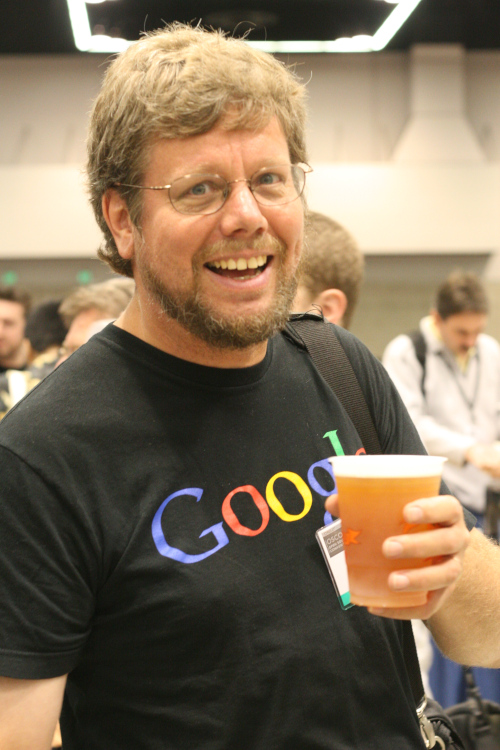
\includegraphics[width = 20mm]{GuidoVanRossumSmall.jpg}
    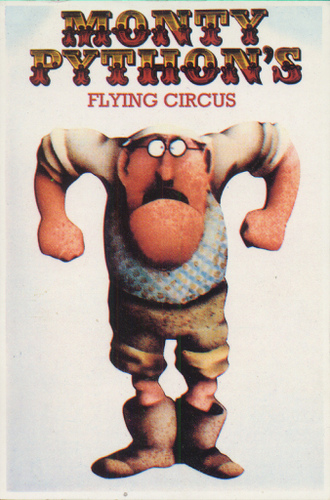
\includegraphics[width = 20mm]{MontyPython.jpg}
\end{center}
    \pause
    \item easy-to-use, highly standardized and with an emphasis on readability of code
\end{itemize}
}


\frame{\frametitle{Why use Python?}
The TIOBE index is a measure of the popularity of programming languages:
    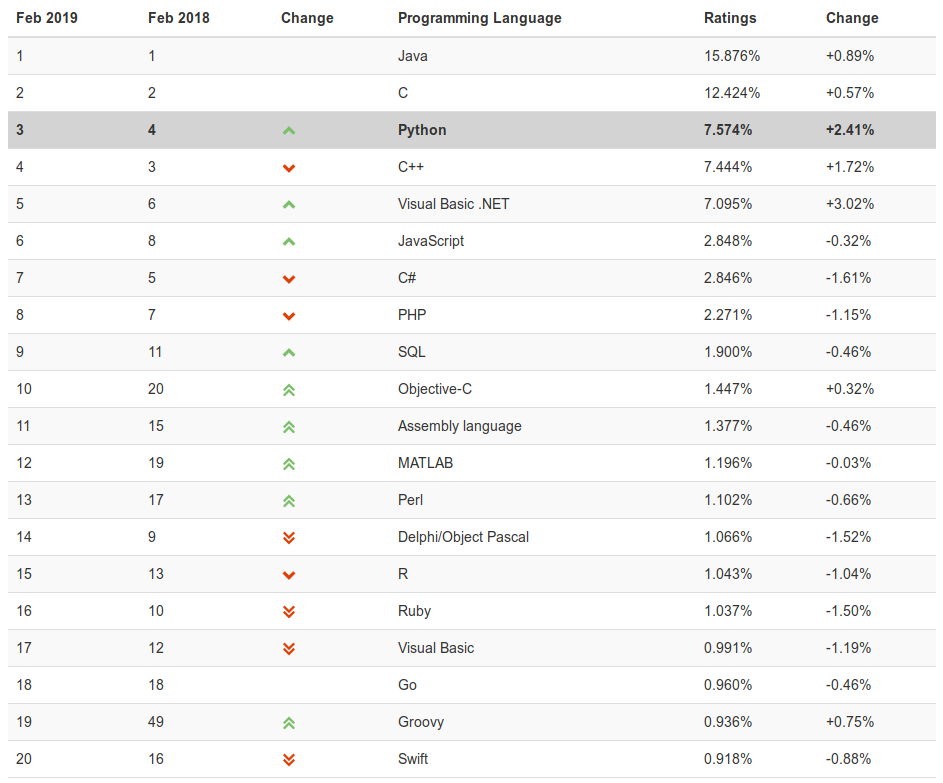
\includegraphics[width = 10cm]{TiobeIndex.png}
}

\begin{frame}{Why Python?}
%. Here are some reasons for its popularity:

\begin{itemize}\addtolength{\itemsep}{0.5\baselineskip}
	\item<1-> It is free! No licence costs
	\item<2-> Runs on all platforms (Mac, Windows, Linux)
	\item<3-> Because of it's ease of programming (e.g no need to worry about memory allocation), Python minimises development effort
	\item<4-> A huge number of \href{https://pypi.python.org/pypi}{libraries}, written by an active \href{https://www.python.org/community/}{community}  
	\item<5-> Python can ``glue" together functions written in C/C++ and Fortran to speed things up (we can also call R and MATLAB functions)
	\item<6-> Compared to other high-level scientific languages such as MATLAB and R, Python offers a much wider range of additional functionality (e.g \href{https://www.djangoproject.com/}{web} and \href{https://wiki.python.org/moin/TkInter}{GUI} development) %hence the nickname ``the swiss army knife" of programming languages. 
\end{itemize}

\end{frame}

%=============================================================================%
%=============================================================================%
\begin{frame}{Horses for courses}

\begin{itemize}\addtolength{\itemsep}{0.5\baselineskip}
	\item<1-> Python is becoming the de facto standard for exploratory and interactive scientific research\\
	\item[]<1-> \textbf{BUT}
	\item<2-> Python is no programming silver bullet
	\item<3-> Your application will ultimately dictate the tool (and a mixture of more than one language \textbf{is} ok). For example:\\
	\begin{itemize}\addtolength{\itemsep}{0.8\baselineskip}
		\item<4-> MATLAB excels at interfacing with hardware, e.g generating \href{https://uk.mathworks.com/products/hdl-coder.html}{hardware description language (HDL) code} to configure an integrated circuit board or connecting to a \href{https://uk.mathworks.com/products/daq.html}{data acquisition card}
		\item<5-> R is great for data wrangling and visualisation, and statistical modelling
        \item<6-> C achieves the fastest runtimes (no wonder why Windows, Mac OS X, Linux have been coded in C (or flavors thereof)), but coding simple things more difficult
	\end{itemize}
\end{itemize}

\end{frame}


\begin{frame}{Why do \textit{you} want to learn Python?}
    Some reasons:
    \pause
    \begin{itemize}
        \item Python has a simple syntax and is widely used; ideal language for beginners
            \pause
        \item Development time is much quicker than for compiled languages like C or Java
            \pause
        \item Broad uptake: Python (and R) have replaced Perl as the key programming language in Bioinformatics
            \pause
        \item Same for spatial applications: major GIS applications like ArcGIS use Python as their main scripting language
        \item Language of choice for machine learning (Tensorflow) 
            \pause
    \end{itemize}
\end{frame}

\frame{\frametitle{Python version 2 vs 3}
    \begin{itemize}
        \item Many systems (e.g., Mac OS X) still use Python 2 as the default
        \item Python 3 differs in \href{https://sebastianraschka.com/Articles/2014\_python\_2\_3\_key\_diff.html}{various ways} from Python 2
        \item Often, Python 3 code cannot be run using a Python 2 interpreter and vice versa
        \item Python 2 is a legacy version and will ultimately be replaced by Python 3
        \item \textbf{Current course will focus on Python 3}
    \end{itemize}
}


\frame{\frametitle{Different Python distributions}
Various distributions of Python available:
    \begin{itemize}
            \pause
        \item Official version from \href{https://python.org}{python.org} 
            \begin{itemize}
                \item Caveat: libraries and other tools need to be installed separately via \texttt{pip}
        \end{itemize}
            \pause
        \item \href{https://www.enthought.com/product/canopy/}{Enthought Canopy}: Python, libraries \& tools in single installer
            \pause
        \item \href{https://www.anaconda.com/distribution/}{Anaconda}: Python, libraries \& tools in single installer: \textbf{used in this course}
            \begin{center}

\includegraphics[width=0.3\textwidth]{AnacondaLogo.png}
            \end{center}
            \pause
    \end{itemize}
}

\frame{\frametitle{Testing small bits of Python code using the IDLE}
IDLE: Integrated Development and Learning Environment
\begin{itemize}
\pause
    \item Windows: Start Menu $>$ Anaconda3 $>$ Anaconda Prompt 
\begin{center}
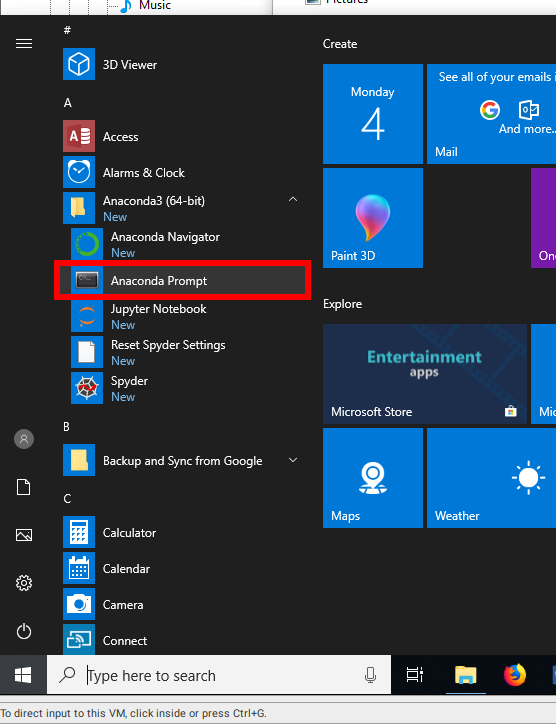
\includegraphics[width=0.3\textwidth]{WindowsStartIDLE.png}
\end{center}
\end{itemize}
}

\frame{\frametitle{Testing small bits of Python code using the IDLE}
\begin{itemize}
    \item In the command-line prompt that appears, type \texttt{python}:
        \pause
    \item You can type Python commands after the \texttt{>>>} mark:
\begin{center}
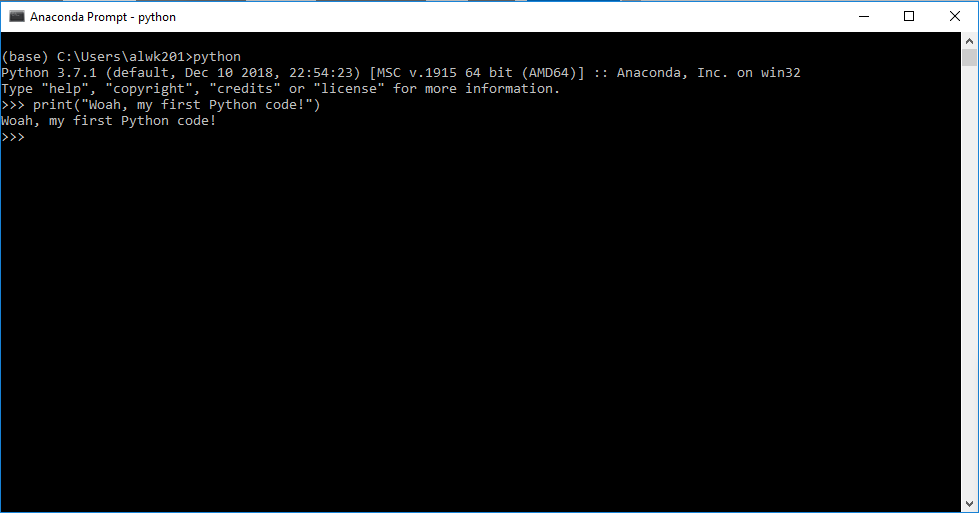
\includegraphics[width=0.75\textwidth]{WindowsAnacondaPrompt.png}
\end{center}
    \item For example, type \texttt{print("Any text you like")}
\end{itemize}
}

\frame{\frametitle{The IDLE interpreter on a Mac}
\begin{itemize}
    \item In Finder, go to Applications $>$ Utilities $>$ Terminal
        \pause
    \item Type \texttt{python3} (not \texttt{python}!) to invoke the IDLE
\begin{center}
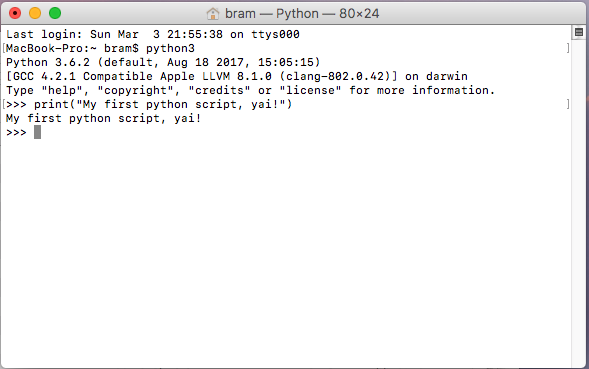
\includegraphics[width=0.5\textwidth]{MacPythonIDLE.png}
\end{center}
    \item IDLE on Linux: open a terminal and type \texttt{python3}
\end{itemize}
}

\frame{\frametitle{IDLE: finding out how things work}
\begin{itemize}
    \item The IDLE prints the value of anything you type back to you
        \pause
    \item This makes the IDLE a great tool to test how commands work
        \pause
    \item Not useful for code that spans multiple lines
\end{itemize}
}


%=============================================================================%
%=============================================================================%
\begin{frame}[fragile]
\frametitle{Executing Python code: IPython interpreter}
\begin{itemize}
	\item IPython is an interactive shell (similar to R Console), adding ``frills" to the vanilla IDLE interpreter, such as:

	\begin{itemize}
		\item syntax highlighting (making it easier to read code)
		\item tab auto-completion (minimises typeos and lists available functions)  
	\end{itemize}
	%\item The IPyton interactive shell is what powers Jupyter in the background (i.e code that I write in these notes is interpreted and executed by the IPython shell)
\end{itemize}

\begin{center}
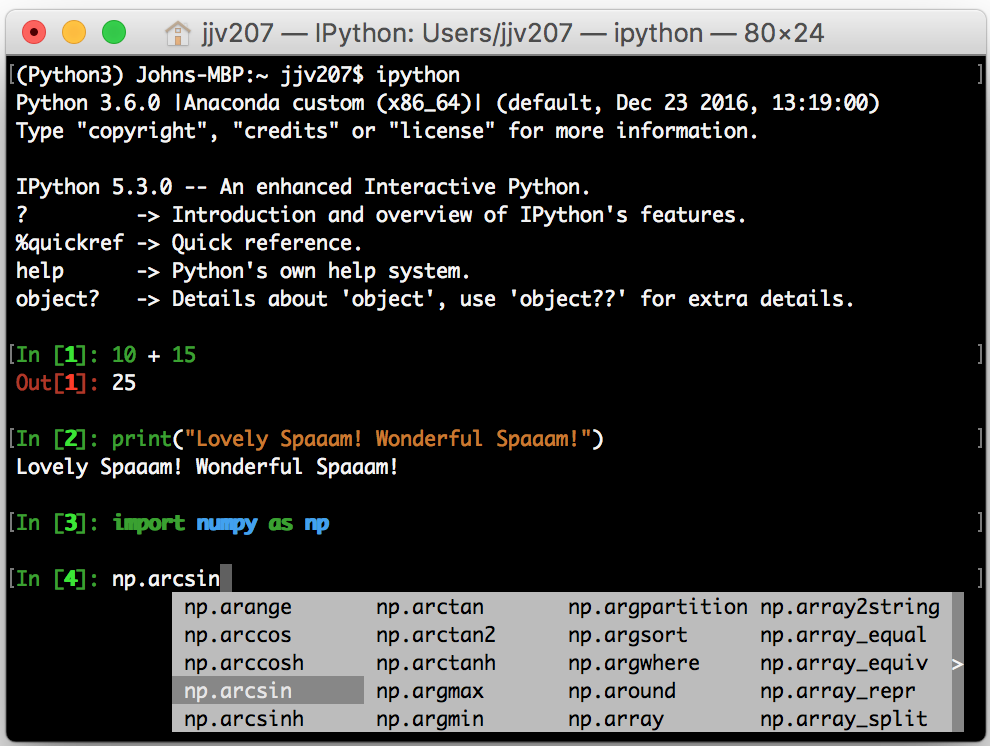
\includegraphics[width=0.6\textwidth]{ipython.png}
\end{center}
\end{frame}

\begin{frame}[fragile]
\frametitle{Executing Python code: Spyder IDE}
    \begin{itemize}
        \item Windows: Start Menu $>$ Anaconda3 $>$ Spyder
            \pause
        \item Mac: Applications $>$ Spyder
    \end{itemize}
\end{frame}

\begin{frame}[fragile]
\frametitle{Executing Python code: Spyder IDE}
\begin{itemize}\addtolength{\itemsep}{.7\baselineskip}
	\item Spyder is an integrated development environment (IDE) for scientific computing, akin to \href{https://www.rstudio.com/}{RStudio} and \href{https://uk.mathworks.com/products/matlab.html}{MATLAB} 
	\item One place to write, execute and debug code, and explore variables
\end{itemize}

\begin{center}
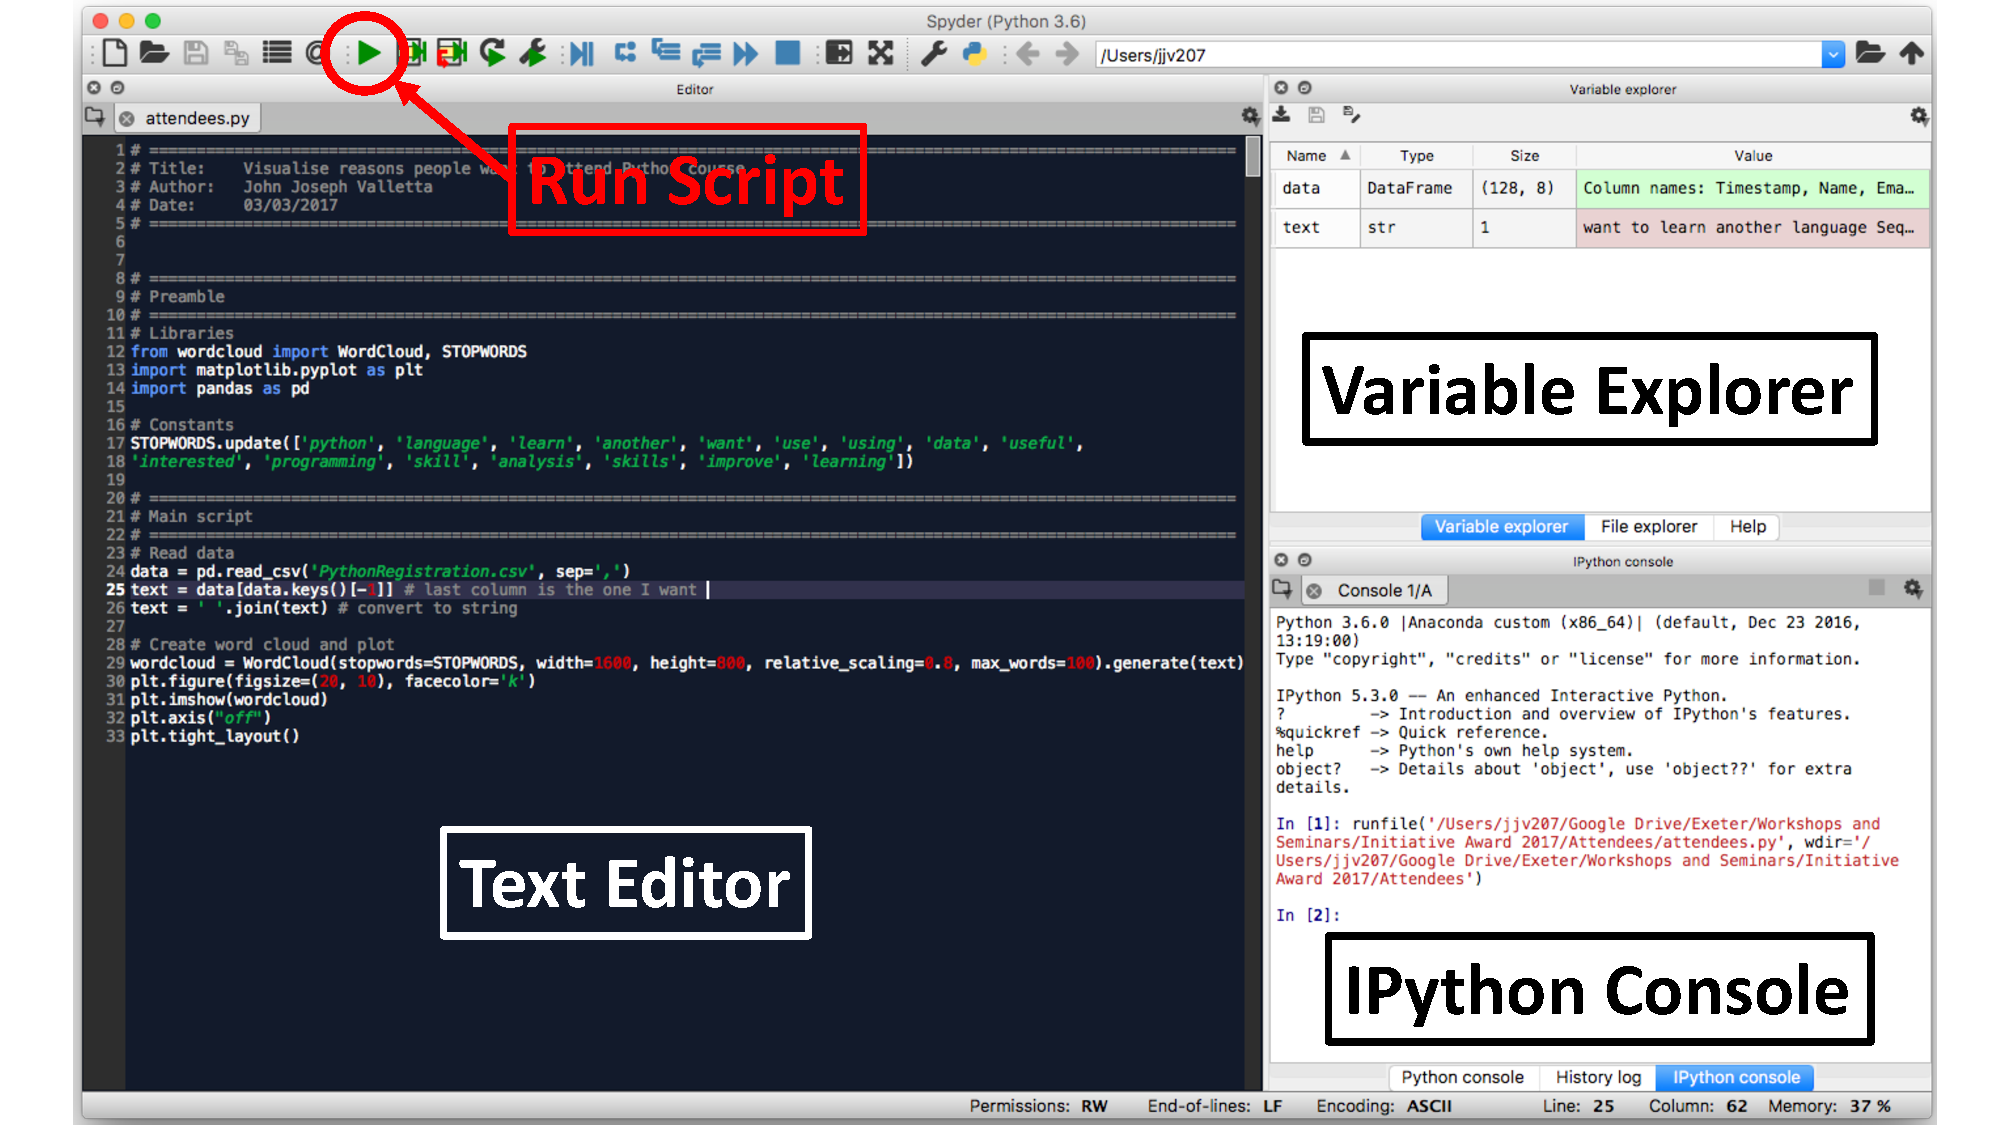
\includegraphics[width=0.8\textwidth]{spyder_annotated.pdf}
\end{center}
\end{frame}

\begin{frame}[fragile]
\frametitle{Running standalone Python scripts without the IDE}
\begin{itemize}
    \item Windows: don't bother, use the Spyder IDE
        \pause
    \item Mac/Linux: 
        \begin{itemize}
            \item Write your code in text file, say \texttt{my\_script.py}
                \pause
            \item In a terminal, run:
\begin{lstlisting}[style=bash]
python3 my_script.py
\end{lstlisting}
        \end{itemize}
\end{itemize}

\end{frame}

\end{document}

